\documentclass[serif,mathserif]{beamer}


\usepackage{fleqn}
%%\usepackage{modefs}
%% \usepackage{math}
\usepackage[utf8]{inputenc}
\usepackage{amsmath, amsfonts, epsfig, xspace}
\usepackage{pstricks,pst-node}
\usepackage{multimedia}
\usepackage[normal,tight,center]{subfigure}
\usepackage{listings}
\setlength{\subfigcapskip}{-.5em}
\usepackage{beamerthemesplit}
\renewcommand\sfdefault{phv}
\renewcommand\familydefault{\sfdefault}
\usetheme{default}
\usepackage{color}
\useoutertheme{default}
\usepackage{texnansi}
\usepackage{marvosym}
\definecolor{bottomcolour}{rgb}{0.32,0.3,0.38}
\definecolor{middlecolour}{rgb}{0.08,0.08,0.16}
\setbeamerfont{title}{size=\Huge}
\setbeamercolor{structure}{fg=gray}
\setbeamertemplate{frametitle}[default]%[center]
\setbeamercolor{normal text}{bg=black, fg=white}
\setbeamertemplate{background canvas}[vertical shading]
[bottom=bottomcolour, middle=middlecolour, top=black]
\setbeamertemplate{items}[circle]
\setbeamerfont{frametitle}{size=\huge}
\setbeamertemplate{navigation symbols}{} %no nav symbols

\author[Vinicius Miana]{Vinicius Miana}

\title[Short Title\hspace{2em}\insertframenumber/\inserttotalframenumber]{Tutorial TableView}

\date{12 de fevereiro de 2014} %leave out for today's date to be insterted

\institute{Universidade Presbiteriana Mackenzie}

\begin{document}


\lstset{language=[Objective]C,
  keywordstyle=\color{blue},
  keywords=[2]{UITableView,UITableViewCell},
  keywordstyle=[2]\color{orange},
  stringstyle=\color{red},
  commentstyle=\color{green},
  breaklines=true,
}

\maketitle

\section{UITableView}  


\begin{frame}
  \frametitle{Desafio: Criar um APP lista de compras}
   Questões:
  \begin{itemize}
  \item Como funciona o UITableView? 
  \item Quais são os componentes envolvidos no seu funcionamento?
  \item Quais são os métodos de uma fonte de dados de uma UITableView?
  \item Como persistir os dados?
  \end{itemize}
\end{frame}


\begin{frame}
  \frametitle{UITableView}
  \begin{itemize}
  \item A UITableView é uma maneira de mostrar e editar uma lista de dados
  \item Seu funcionamento depende de uma fonte de dados: UITableViewDataSource e de um delegate: UITableViewDelegate
  \item Uma das maneiras de fazer isso é através de uma sub-classe do UITableViewController  
  \end{itemize}
\end{frame}



\begin{frame}
  \frametitle{UITableViewDataSource}
  \begin{itemize}
  \item Veja quais são os métodos do protocolo UITableViewDataSource
  \item Clone o projeto lista de compras e verifique como estão implementados
  \item Pense em como usar estes métodos para acessar uma lista de compras que está armazenada no NSUserDefaults
  \item Crie uma classe ItemCompra para representar um item a ser comprado com atributos: nome e quantidade  
  \end{itemize}
\end{frame}



\begin{frame}[fragile]
  \frametitle{Reutilização de Células}
  Para otimizar o uso da mémoria podemos reutilizar as células
  \begin{lstlisting}
    - (UITableViewCell *)tableView:(UITableView *)tableView cellForRowAtIndexPath:(NSIndexPath *)indexPath
    {
      UITableViewCell *cell = [tableView dequeueReusableCellWithIdentifier:@"Cell"];
      if(!cell) {
        cell = [[UITableViewCell alloc] initWithStyle:UITableViewCellStyleDefault reuseIdentifier:@"Cell"];
      }
      // Get the data from the database and fill the cell
      return cell;
    }  
  \end{lstlisting}
\end{frame}

\begin{frame}
  \frametitle{Estilos das células}
  A células de um TableView podem ser customizadas através de 4 opções pré-definidas:
  UITableViewCellStyleDefault (Basic no storyboard), UITableViewCellStyleValue1 (RightDetail),
  UITableViewCellStyleValue2 (LeftDetail),
  UITableViewCellStyleSubtitle (Subtitle) que estão respectivamente representados na figura
  \begin{figure}[t]
    \centering
    \subfigure[Exemplos de estilo de células]{
      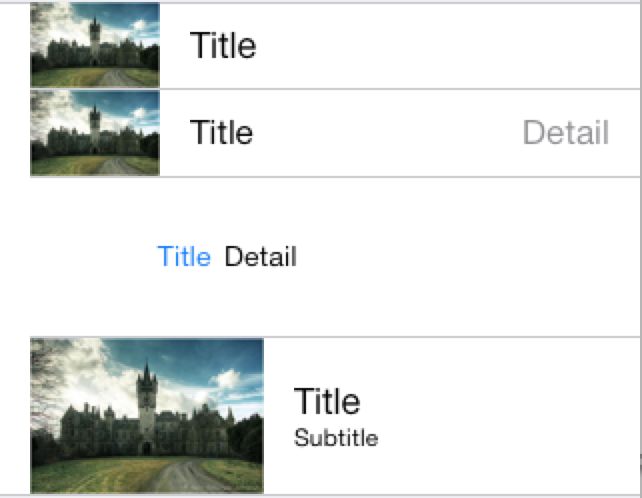
\includegraphics[width=5cm]{img/tableCellStyles.png}
    }
  \end{figure}
\end{frame}





\begin{frame}
  \frametitle{Questions}
\end{frame}
\end{document}
